
%(BEGIN_QUESTION)
% Copyright 2010, Tony R. Kuphaldt, released under the Creative Commons Attribution License (v 1.0)
% This means you may do almost anything with this work of mine, so long as you give me proper credit

This DP transmitter measures the pressure drop developed by an orifice plate as a hydrocarbon liquid ($\gamma$ = 47 lb/ft$^{3}$) flows through the pipe.  The orifice plate flow range is 0 to 550 GPM and its corresponding differential pressure range is 0 to 125 inches H$_{2}$O:

$$\includegraphics[width=15.5cm]{i03731x01.eps}$$

Normally, high-density glycol (S.G. = 1.8) is pumped into both impulse lines to completely fill them and displace any light hydrocarbon liquid that might otherwise collect there.  Unfortunately, some of this fill fluid has leaked out of the low-side impulse line, so that only 30 out of its 34 vertical inches of height are filled with glycol, the upper 4 inches filled with process liquid.  The high-side impulse line still has all of its fill fluid intact.

\vskip 10pt

Calculate the amount of differential pressure this filling error will impart to the DP transmitter, and then calculate how much flow the transmitter will ``think'' is going through the pipe as a result of this false pressure difference when in fact the flow is completely stopped.

\vskip 30pt

DP error = \underbar{\hskip 50pt} inches H$_{2}$O

\vskip 30pt

Flow error (at zero flow) = \underbar{\hskip 50pt} GPM

\vfil 

\underbar{file i03731}
\eject
%(END_QUESTION)





%(BEGIN_ANSWER)

This is a graded question -- no answers or hints given!

%(END_ANSWER)





%(BEGIN_NOTES)

With both impulse lines equally filled, the amount of {\it hydrostatic} differential pressure at the transmitter will be zero (i.e. the hydrostatic pressure of each line will be equal in magnitude, and opposite in effect at the transmitter).  However, if some of the dense glycol leaks out and is replaced by lighter process fluid, it will cause the impulse lines' hydrostatic pressures to be unequal.

\vskip 10pt

One may calculate this difference by first calculating the hydrostatic pressure generated by the full impulse line (34 inches at a specific gravity of 1.8) and then subtract the hydrostatic pressure generated by the partially full impulse line (30 inches of heavy glycol plus 4 inches of light process fluid).  The more mathematically astute will see that a quicker way is to simply multiply the 4 inches of unfilled impulse line by the difference in specific gravities:

$$\hbox{DP error } = (4 \hbox{ in}) \left(1.8 - {47 \hbox{ lb/ft}^3 \over 62.4 \hbox{ lb/ft}^3} \right) = 4.187 \hbox{ "WC}$$

This error of 4.187 "WC (a positive differential pressure, as the ``high'' port sees more pressure than the ``low'' port) causes the transmitter to register a positive flow even when none exists.  To calculate how much flow is equivalent to 4.187 "WC of differential pressure, we may set up the standard volumetric flow equation ($Q = k \sqrt{\Delta P}$), solve for $k$ in this application, and then solve for $Q$:

$$Q = k \sqrt{\Delta P}$$

$$550 = k \sqrt{125}$$

$$k = 49.193$$

\vskip 10pt

$$Q = k \sqrt{\Delta P}$$

$$Q = 49.193 \sqrt{4.187}$$

$$Q = 100.66 \hbox{ GPM}$$

\vskip 10pt

Therefore, this flowmeter will falsely register a flow rate of 100.66 gallons per minute when there is actually no flow going through the pipe!

%INDEX% Measurement, flow: orifice plate

%(END_NOTES)

